\section{Application Programmer Interface (API)}

The ThreadPool manages a set of parallel threads running on the local computational node and sharing the resources of that computational node.
%
An application can dispatch thread-parallel work, defined by a work subprogram and work information, to the ThreadPool.
%
The ThreadPool causes each parallel thread, including the application's \emph{main} thread, to call the application's work subprogram with the application's work information.
%
The ThreadPool application programmer interface (API), ThreadPool implementation, and application's work subprograms conform to the standard C programming language.


The ThreadPool has four states: NULL, BLOCKED, READY, and ACTIVE.
%
These states and state transitions are illustrated in the ThreadPool state diagram given in Figure~\ref{fig:ThreadPoolStates}.
%
Each state transition occurs through application calls to the ThreadPool functions noted in Figure~\ref{fig:ThreadPoolStates}.
%
\begin{figure}[h]
\begin{center}
\fbox{
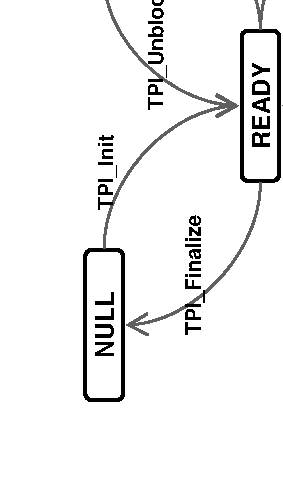
\includegraphics[viewport=0.5in 0.5in 2.75in 4.75in,angle=270,scale=1]{figures/StateDiagram}
}
\caption{ThreadPool state diagram with state transitions identified by thread pool functions}
\label{fig:ThreadPoolStates}
\end{center}
\end{figure}

The ThreadPool is in the ACTIVE state while running an application's work subprogram.
%
A work subprogram may be run in several different thread-parallel modes,
as described in Sections~\ref{sec:RunWork}-\ref{sec:WorkSubprogramWithReduce}.
%
An application selects the thread-parallel mode by calling the associated version of a
\texttt{TPI\_Run\_*} function.


\clearpage
\subsection{Initialization, Finalization, and Blocking}

\subsubsection{TPI\_Init( int thread\_count )}

The ThreadPool starts in the NULL state, without any additional threads of execution.
%
An application calls the \texttt{TPI\_Init} function to create \texttt{thread\_count-1} threads and transition the ThreadPool from the NULL state to the READY state.
%
This \texttt{TPI\_Init} function can only be called when the ThreadPool is in the NULL state.
%
These created threads are in addition to the application's \emph{main} thread, for a total of
\texttt{thread\_count} available threads of execution.
%
While in the READY state the ThreadPool is ready to dispatch work routine to threads.


Thread creation and initialization is a time consuming operation.
%
As such the ThreadPool creates threads during initialization and then holds them in the READY state for subsequent use by the application.
%
Threads in the READY state are continually running on the manycore CPU and polling the ThreadPool for work to be performed.
%
This strategy minimizes the time required to dispatch work to threads by maintaining the threads in this \emph{ready to run} state.


It is recommended that the number of requested threads, \texttt{thread\_count}, be no greater than the number of available processing cores.
%
If more threads are requested then the threads will be required to block and unblock
(\emph{i.e.}, context switch) in order for all of the threads to execute.
%
This blocking and unblocking introduces overhead which degrades thread-parallel performance.


\subsubsection{TPI\_Finalize()}

While in the READY state an application calls \texttt{TPI\_Finalize} to destroy the created threads and transition the ThreadPool to the NULL state.
%
A call to \texttt{TPI\_Finalize} can be followed by a call to \texttt{TPI\_Init} to reinitialize the ThreadPool with a different number of threads.


\subsubsection{TPI\_Block() and TPI\_Unblock()}

While in the READY state the created threads are running and consuming CPU resources.
%
If an application creates additional non-ThreadPool threads, either explicitly or through a different parallel threading library, the ThreadPool threads in the READY state will continually compete with those non-ThreadPool threads for CPU resources.
%
An application may block the ThreadPool created threads to preempt this competition for CPU resources.
%
The \texttt{TPI\_Block()} blocks the ThreadPool created threads and transitions the ThreadPool from the READY state to the BLOCKED state.


An application unblocks the ThreadPool created threads by calling \texttt{TPI\_Unblock()}.
%
This function returns the ThreadPool to the READY state with the ThreadPool created threads running and polling the ThreadPool for work.
%
Blocking and unblocking created threads is a time consuming operation; however, it is not as time consuming as destruction and creation of threads.


\subsubsection{Intended Use}

An application code initializes the ThreadPool, calls a sequence of algorithms, and then finalizes the ThreadPool.
%
An algorithm is assumed to run many thread-parallel computational kernels through a single threading mechanism; \emph{e.g.}, ThreadPool, OpenMP, or TBB.
%
An algorithm which runs computational kernels through the ThreadPool mechanism would unblock the worker threads, run its sequence of thread-parallel computational kernels, and then return the worker threads to the blocked state.
%
This assumed application and algorithm flow is summarized in Figure~\ref{fig:WorkFlow}.

\begin{figure}[h]
\center
\small
\begin{boxedverbatim}
#include<TPI.h>

int main(...)
{
  TPI_Init( thread_count );
  /*
   *  Application's program control flow
   *  calls application's algorithms.
   */
  TPI_Finalize();
}

void an_application_algorithm(...)
{
  const int was_blocked = TPI_Isblocked();
  if ( was_blocked ) TPI_Unblock();
  /*
   *  Run many thread-parallel computational kernels...
   */
  if ( was_blocked ) TPI_Block();
  return ;
}
\end{boxedverbatim}
\caption{Assumed work flow for an application and its algorithms}
\label{fig:WorkFlow}
\end{figure}


%--------------------------------------------------------------------------------
\clearpage
\subsection{Running Work Subprograms} \label{sec:RunWork}

While in the READY state an application calls one of the \texttt{TPI\_Run} functions to dispatch  work subprograms to be called on all available threads, including the application's main thread.
%
A \texttt{TPI\_Run} function can only be called when the ThreadPool is in the READY state.
%
While an application's work subprogram is running the ThreadPool is in the ACTIVE state.
%
When all invocations of the work subprogram return, the ThreadPool returns to the READY state.



\subsubsection{Work Subprogram}

An application's work subprogram is called by the ThreadPool an application-specified number of times.
%
Each call to the work subprogram is responsible for performing an application-specified portion of the computational work.
%
Two pieces of information is required by a call to the work subprogram:
(1) the computational work to be performed and
(2) a means of partitioning this work.


An application's work subprogram is a function conforming to the C language interface defined in Figure~\ref{fig:WorkSubprogram}.
%
A work subprogram determines which portion of work that it should perform from members of the input
\texttt{TPI\_Work\_Struct} argument.
%
\begin{figure}[h]
\center
\small
\begin{boxedverbatim}
struct TPI_Work_Struct {
  const void * info ;       /**< Shared info input to TPI_Run         */
  void       * reduce ;     /**< Data for reduce operation, if any    */
  int          count ;      /**< Count of work requested via TPI_Run  */
  int          rank ;       /**< Rank  of work for the current call   */
  int          lock_count ; /**< Count of locks requested via TPI_Run */
};

typedef const struct TPI_Work_Struct TPI_Work ;

typedef void (*TPI_work_subprogram)( TPI_Work * work );
\end{boxedverbatim}
\caption{TPI work subprogram C language interface defined in the \texttt{TPI.h} header file}
\label{fig:WorkSubprogram}
\end{figure}
%
\begin{blist}
\item The \texttt{work->info} member provides a pointer to application-provided work information.  This work information is shared by all calls to a work subprogram on all threads.  It is declared constant to promote safe multi-threaded access.
%
\item The \texttt{work->count} member identifies the total number times the work subprogram is being called during a single call to a \texttt{TPI\_Run} function.
%
\item The \texttt{work->rank} member is given a unique value for each call of the work subprogram.  These values are in the range \mbox{[0..\texttt{work->count}-1]}.
Due to non-determinism of thread-execution there is no guaranteed correlation between the
\texttt{work->rank} value and the calling order of the work subprogram.
These \texttt{work->rank} and \texttt{work->count} members provide the minimal information required for a call to a work subprogram to determine its portion of the total work to be performed.
%
\end{blist}
%
The remaining \texttt{TPI\_Work\_Struct} members are described with respect to the calling \texttt{TPI\_Run} functions.

\clearpage
\subsubsection{Calling Work Subprograms via TPI\_Run\_threads(\ldots)}

\begin{center}
\small
\begin{boxedverbatim}
int TPI_Run_threads( TPI_work_subprogram work_subprogram  ,
                     const void *        work_info ,
                     int                 lock_count /* = 0 */ );
\end{boxedverbatim}
\end{center}

The \texttt{TPI\_Run\_threads} function is used to call an application's work subprogram
once on each available thread, both main and created threads.
%
A simple use of this function to perform a thread-parallel \mbox{$Y=\alpha*X+Y$} operation is illustrated in Figure~\ref{fig:WorkSubprogramAXPY}.

\begin{figure}[h]
\small
\center
\begin{boxedverbatim}
typedef struct {
  int n ;
  double a ;
  double * x ;
  double * y ;
} WorkInfo ;

void daxpy( int n , double a , double * x , double * y )
{
  WorkInfo work_info = { n , a , x , y };
  TPI_Run_threads( tpi_daxpy , & work_info , 0 );
}
void tpi_daxpy( TPI_Work * work )
{
  const WorkInfo * const info = (const WorkInfo *) work->info ;
  int begin , end , i ;
  compute_span_of_work( work->count , work->rank , info->n , & begin , & end );
  for ( i = begin ; i < end ; ++i ) {
    work->y[i] += work->a * work->x[i] ;
  }
}
\end{boxedverbatim}
\caption{Example implementation of a simple, thread parallel AXPY operation using \texttt{TPI\_Run\_threads}}
\label{fig:WorkSubprogramAXPY}
\end{figure}


When the application's work subprogram is called by each thread the \texttt{TPI\_Work} argument (see Figure~\ref{fig:WorkSubprogram}) is populated with the following information.
%
\begin{blist}
\item \texttt{work->info} = pointer to \texttt{work\_info} --- the application-supplied \emph{shared} work data,
\item \texttt{work->count} = the total number of threads calling the work subprogram, and
\item \texttt{work->rank} = the rank of the calling thread.
\end{blist}

\clearpage
\subsubsection{Calling Work Subprograms via TPI\_Run(\ldots)}

\begin{center}
\small
\begin{boxedverbatim}
int TPI_Run( TPI_work_subprogram work_subprogram  ,
             const void *        work_info ,
             int                 work_count  ,
             int                 lock_count /* = 0 */ );
\end{boxedverbatim}
\end{center}

An application can specify that the work subprogram is called \texttt{work\_count} times, regardless of the number of available threads.
%
The ThreadPool threads use an internally-shared work counter to guarantee the correct number of calls, and to provide a unique \texttt{work->rank} for each call.
%
In this interface the \texttt{TPI\_Work\_Struct} is populated with the following information.
%
\begin{blist}
\item \texttt{work->info} = pointer to \texttt{work\_info} --- the application's \emph{shared} work data,
\item \texttt{work->count} = \texttt{work\_count} --- the specified number of calls to the work subprogram, and
\item \texttt{work->rank} = the rank of the call out of the specified number of calls.
\end{blist}



This interface is intended for applications that
(1) have a large amount of work to perform and
(2) have units of work with an irregular computational load.
%
In this situation the application can partition its irregular work into many more units of work that there are threads, and then dispatch the work subprogram to process these \texttt{work\_count} units of work.
%
As each thread completes a call to the application's work subprogram it will claim the next unit of work from the shared work counter.


This interface provides an application with a means for automatically (but only approximately) balancing computational work among threads.
%
The quality of this load balancing is dependent upon the the variability of the work load among the units of work.


\subsection{Running Work Subprograms with Locks} \label{sec:RunWorkLock}

When a work subprogram updates a shared variable or data structure that update must be thread safe.
%
One strategy for thread safe updates is with \emph{mutually exclusive locks}
(referred to as \emph{mutex} in the \textbf{pthreads} API).
%
Locks provide mutually exclusive execution of those portions of a work subprogram that access a shared variable or data structure that is updated by the work subprogram.
%
This usage is illustrated by the simple, thread-parallel implementation of a dot product given in Figure~\ref{fig:WorkSubprogramDDOTlocking}.

\begin{figure}[h]
\small
\center
\begin{boxedverbatim}
typedef struct {
  int n ;
  double * result_pointer ;
  const double * x ;
  const double * y ;
} WorkInfo ;

double ddot( int n , const double * x , const double * y )
{
  double result = 0.0 ;
  WorkInfo work_info = { n , & result , x , y };
  TPI_Run_threads( tpi_ddot , & work_info , 1 /* lock_count */ );
  return result ;
}
void tpi_ddot( TPI_Work * work )
{
  const WorkInfo * const info = (const WorkInfo *) work->info ;
  double local_result = 0.0 ;
  int begin , end , i ;
  compute_span_of_work( work->count , work->rank , info->n , & begin , & end );
  for ( i = begin ; i < end ; ++i ) {
    local_result += work->y[i] * work->x[i] ;
  }
  TPI_Lock(0);                              /* probable blocking */
  *(work->result_pointer) += local_result ; /* serialized */
  TPI_Unlock(0);
}
\end{boxedverbatim}
\caption{Example implementation for a simple, thread parallel DDOT operation using \texttt{TPI\_Run\_threads}, \texttt{TPI\_Lock}, and \texttt{TPI\_Unlock}}
\label{fig:WorkSubprogramDDOTlocking}
\end{figure}

In the illustrative implementation (Figure~\ref{fig:WorkSubprogramDDOTlocking}), each thread-parallel call to \texttt{tpi\_ddot} has its own thread-local accumulation variable \texttt{local\_result}.
%
Summation of the local accumulation into the global accumulation is thread safe by the calls to \texttt{TPI\_Lock} and \texttt{TPI\_Unlock}.
%
The first thread to arrive at \texttt{TPI\_Lock} acquires the mutually exclusive lock and proceeds with the local-to-global accumulation.
%
If a second thread arrives at this function call it will block and wait for the first thread to release the lock via \texttt{TPI\_Unlock}.
%
Once the first thread releases the lock the second thread unblocks, acquires the lock, and proceeds with its own contribution to the summation.


Using mutually exclusive locks has the performance liabilities of
\begin{blist}
\item serializing thread execution between \texttt{TPI\_Lock} and \texttt{TPI\_Unlock},
\item introducing overhead for blocking and unblocking threads, and
\item introducing a non-deterministic race condition for the local-to-global accumulation.
\end{blist}
%
The serialization and overhead liabilities increase execution time.
%
The non-deterministic liability can cause computions to be non-repeatable.
%
All of these liabilities can be addressed for reduction operations through the following section.


\clearpage
\subsection{Running Work Subprograms with Reductions} \label{sec:WorkSubprogramWithReduce}

Alternate versions of the \texttt{TPI\_Run} and \texttt{TPI\_Run\_threads} functions,
\texttt{TPI\_Run\_reduce} and \texttt{TPI\_Run\_threads\_reduce} respectively,
are defined to support efficient reduction operations.
%
An example usage of this reduction-supporting interface is given in
Figure~\ref{fig:WorkSubprogramDDOTreduce}.

\begin{center}
\small
\begin{boxedverbatim}
typedef void (*TPI_reduce_init)( TPI_Work * work );
typedef void (*TPI_reduce_join)( TPI_Work * work , const void * reduce );

int TPI_Run_threads_reduce( TPI_work_subprogram work_subprogram  ,
                            const void *        work_info ,
                            TPI_Reduce_join     reduce_join ,
                            TPI_Reduce_init     reduce_init ,
                            int                 reduce_size ,
                            void *              reduce_data );

int TPI_Run_reduce( TPI_work_subprogram work_subprogram  ,
                    const void *        work_info ,
                    int                 work_count  ,
                    TPI_Reduce_join     reduce_join ,
                    TPI_Reduce_init     reduce_init ,
                    int                 reduce_size ,
                    void *              reduce_data );
\end{boxedverbatim}
\end{center}

\paragraph{\texttt{work->reduce}:}
%
Each call to the \texttt{work\_subprogram} accumulates its portion of the reduction operation into a reduction variable, pointed to by the \texttt{work->reduce} argument.
%
Each call to the \texttt{work\_subprogram} has exclusive access to the reduction variable --- no locking is required.
%
Exclusive access is guaranteed by each thread having its own copy of the reduction variable.
%
This copy is allocated to be \texttt{reduce\_size} bytes and is initialized by a call to the application-provided \texttt{reduce\_init} function.


\paragraph{\texttt{reduce\_join}:}
%
As threads complete their calls to the \texttt{work\_subprogram} the per-thread reduction variables are reduced (joined together) via the application's \texttt{reduce\_join} function.
%
The final result is reduced into the application-provided reduction variable pointed to by the \texttt{reduce\_data} argument.
%
These join operations occur without additional serialization, without extra runtime overhead, and are deterministic.
%
Thus for algorithms with reduction operations, or with updates to shared variables which can be expressed as reduction operations, this interface resolves the performance liabilities of the locking / unlocking approach.



\begin{figure}[ht]
\small
\center
\begin{boxedverbatim}
typedef struct {
  int n ;
  const double * x ;
  const double * y ;
} WorkInfo ;

double ddot( int n , const double * x , const double * y )
{
  double result = 0.0 ;
  WorkInfo work_info = { n , & result , x , y };
  TPI_Run_threads_reduce( tpi_ddot , & work_info ,
                          tpi_ddot_join , tpi_ddot_init ,
                          sizeof(result) , & result );
  return result ;
}
void tpi_ddot( TPI_Work * work )
{
  const WorkInfo * const info = (const WorkInfo *) work->info ;
  double * const local_result = (double*) work->result ;
  int begin , end , i ;
  compute_span_of_work( work->count , work->rank , info->n , & begin , & end );
  for ( i = begin ; i < end ; ++i ) {
    *local_result += work->y[i] * work->x[i] ;
  }
}
void tpi_ddot_join( TPI_Work * work , const void * reduce )
{ *((double*) work->reduce) += *((const double*) reduce); }

void tpi_ddot_init( TPI_Work * work }
{ *((double*) work->reduce) = 0 ; }
\end{boxedverbatim}
\caption{Example implementation of a simple, thread parallel DDOT operation using \texttt{TPI\_Run\_threads\_reduce}}
\label{fig:WorkSubprogramDDOTreduce}
\end{figure}


